\documentclass[conf]{new-aiaa}
%\documentclass[journal]{new-aiaa} for journal papers
\usepackage[utf8]{inputenc}

\usepackage{graphicx}
\usepackage{amsmath}
\usepackage{commath}
\usepackage[version=4]{mhchem}
\usepackage{siunitx}
\usepackage{longtable,tabularx}
\usepackage{float}
\usepackage{listings}
\usepackage{pdfpages}
\usepackage{color} %red, green, blue, yellow, cyan, magenta, black, white
\definecolor{mygreen}{RGB}{28,172,0} % color values Red, Green, Blue
\definecolor{mylilas}{RGB}{170,55,241}
\setlength\LTleft{0pt} 

\lstset{language=Matlab,%
	basicstyle=\footnotesize,
	breaklines=true,%
	morekeywords={matlab2tikz},
	keywordstyle=\color{blue},%
	morekeywords=[2]{1}, keywordstyle=[2]{\color{black}},
	identifierstyle=\color{black},%
	stringstyle=\color{mylilas},
	commentstyle=\color{mygreen},%
	showstringspaces=false,%without this there will be a symbol in the places where there is a space
	numbers=left,%
	numberstyle={\tiny \color{black}},% size of the numbers
	numbersep=9pt, % this defines how far the numbers are from the text
	emph=[1]{for,end,break},emphstyle=[1]\color{red}, %some words to emphasise
	%emph=[2]{word1,word2}, emphstyle=[2]{style},    
}

% ================================================================ % 
\title{ASE387P.2 Mission Analysis and Design \\ Homework 2}

\author{Junette Hsin}
\affil{Masters Student, Aerospace Engineering and Engineering Mechanics, University of Texas, Austin, TX 78712}

\begin{document}

\maketitle

% \begin{abstract}

	% The theory and algorithms are derived and computer program to establish the trajectory of
	% an Earth-orbiting satellite is developed. The assumptions for the study are ...

% \end{abstract}
% ================================================================ % 
% THIS IS A TEST 

\begin{equation}
    e^{i \theta} = cos(\theta) + i sin(\theta)
\end{equation}

\begin{equation}
    cos(\vartheta) = cos^2(i_{init}) sin^2(i_{init}) cos( \Delta \Omega )
\end{equation}

\begin{equation}
    cos(u_{init}) = tan(i_{init}) \dfrac{ cos( \Delta \Omega ) - sin( \vartheta ) }{sin( \vartheta )}
\end{equation}

\begin{equation}
    cos(u_{fin}) = cos(i_{init}) sin(i_{init}) \dfrac{ 1 - cos(\Delta \Omega) }{sin(\vartheta)}
\end{equation}

\begin{equation}
    \Delta v_{unit} = v_{fin} - v_{init}
\end{equation}

\begin{equation}
    \Delta v_{mag} = 2 \dfrac{||v_{init}||}{sin(\vartheta)}
\end{equation}

\begin{equation}
    \Delta i = i_{fin} - i_{init}
\end{equation}

\begin{equation}
    h = r \times v 
\end{equation}

\begin{equation}
    tan(\phi_{fpa}) = e \dfrac{sin(\nu)}{1 + e cos(\nu)}
\end{equation}

\begin{equation}
    \Delta v_{mag} = 2 || v_{init} || cos(\phi_{fpa}) sin(\frac{\Delta i}{2})
\end{equation}

\begin{equation}
    \Delta v = \Delta v_{mag} h_{unit}
\end{equation}

% ================================================================ % 

\newpage 
% ================================================================ % 
\section*{Problem 1}

% Statement 
Consider the possible transfer orbits from Earth to
Mars. Assume both planets are in coplanar circular heliocentric orbits. Consider a transfer
angle of 75°. 

% 1.a 
\subsection*{A}

Choose a range of semi-major axes up to a distance of 2 A.U. and draw a plot (to
scale) of the semi-major axes (X-axis) versus time-of-flight (Y-axis) of the
transfer orbit. Note that there are two possible times for flight for each transfer
orbit semi-major axis – the short-way and the long-way.

\subsubsection*{Solution}

\begin{figure}[H]
	\centering 
	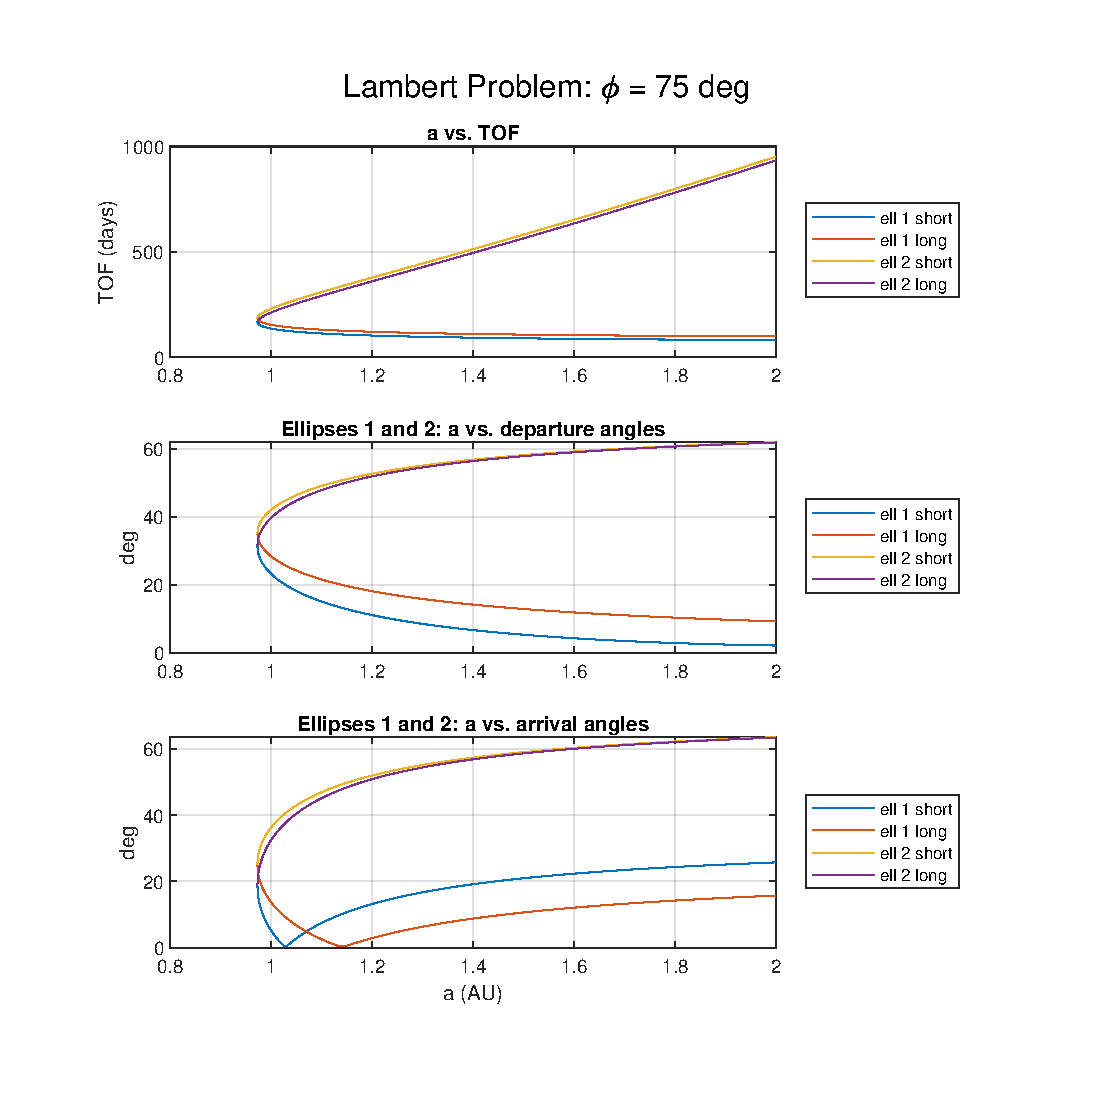
\includegraphics[width=0.8\textwidth]{phi75_Ellipse 1 and 2 TOF and Angles.pdf}
	\caption{TOF and Departure/Arrival Angles vs. a}
	\label{fig:TOF_angles_a}
\end{figure}



\begin{figure}[H]
	\centering 
	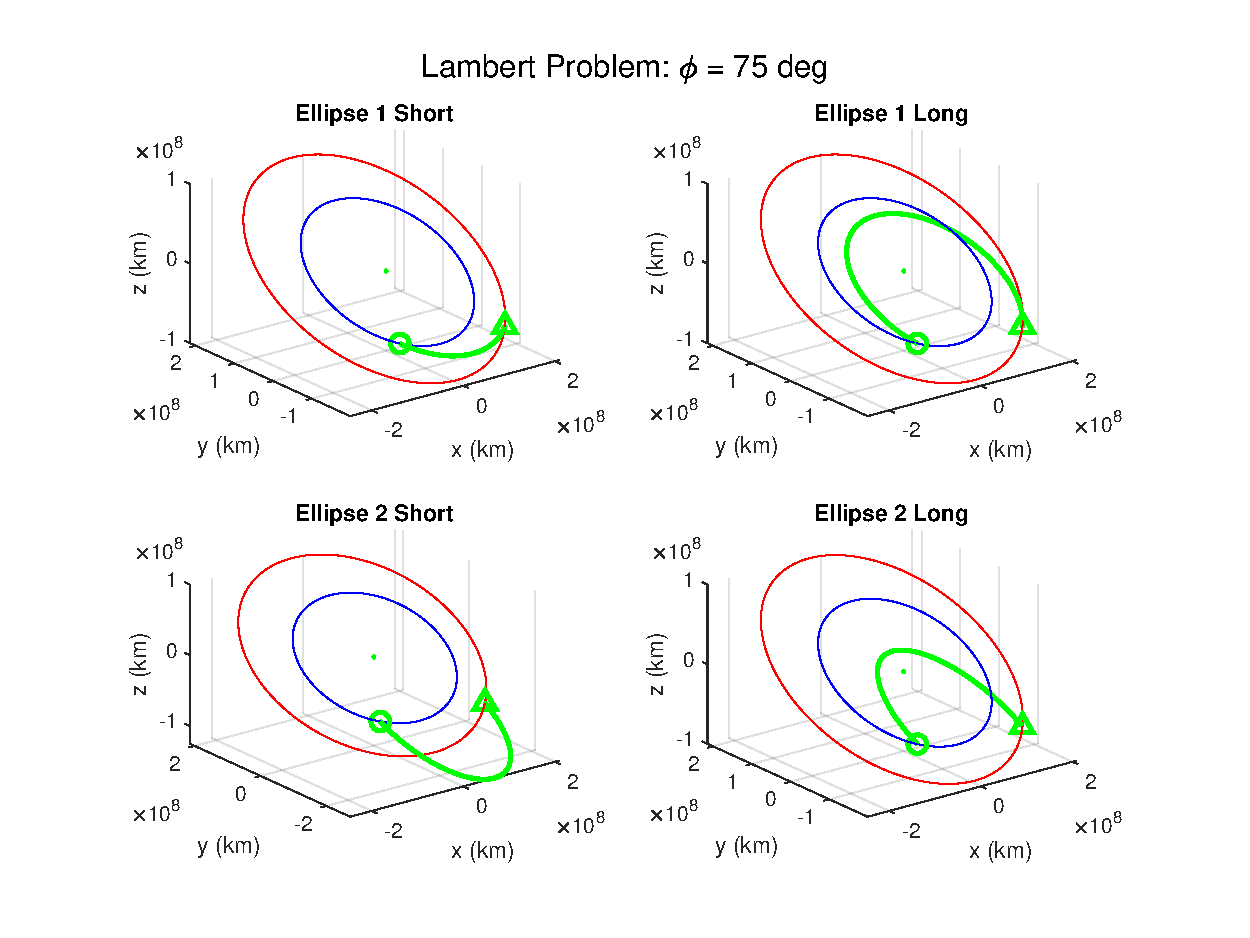
\includegraphics[width=0.8\textwidth]{orbits_Ellipse 1 and 2, Short and Long.pdf}
	\caption{Visualization of Transfer Orbits}
	\label{fig:transfer_orbits}
\end{figure}

(Bonus) Figure \ref{fig:transfer_orbits} visualizes the transfer orbits for both ellipses. The red orbit represents Mars and the blue orbit represents Earth. The green circles indicate the initial departure position and the green triangles indicate the final arrival position. The green lines map out the trajectory of the probe on its path to Mars. 

% 1.b 
\subsection*{B}
What is the value of the semi-major axis and eccentricity for the minimum energy
transfer orbit?

\subsubsection*{Solution}

$A_{min}$ = 0.97301 AU and $e_{min}$ = 0.53129. 

% 1.c 
\subsection*{C}
For the given transfer angle and for any chosen semi-major axis, at the departure
and arrival points, calculate the angles between the velocity of the probe and the
velocity of the departure and arrival planets, respectively. Let us call these
“departure angle” and “arrival angle” – this may be non-standard terminology.
We have two of each – one for short-way travel and another for long-way travel.

\subsubsection*{Solution}

Please see Figure \ref{fig:TOF_angles_a}. The Battin Method from Vallado (Fundamentals of Astrodynamics and Applications, ed. 4) was used to calculate the velocity vectors and angles for the departure and arrival positions. 

% 1.d 
\subsection*{D}
Plot the departure and arrival angles for this case as a function of the transfer orbit
semi-major axis.

\subsubsection*{Solution}

Please see Figure \ref{fig:TOF_angles_a}. 

% 1.e 
\subsection*{E}
Discuss the significance of these plots for decision-making on the choice of semimajor axes for the fixed transfer angle.

\subsubsection*{Solution}

Lower departure and arrival angles may be desirable for a mission, as the delta-V required to enable capture by the destination planet's gravity would be lower. Balancing the desirability of a spacecraft orbit versus costs such as fuel expenditure needs to be evaluated.  


% \newpage 
% ================================================================ % 
\section*{Problem 2}

Repeat Problem 1 for 15° increments of the transfer angle, that is for [15, 30,45, 60, 75,
90, 105, 120, 135, 150, 165, 180] degrees.

% 2.a 
\subsection*{A}
Plot the departure angle, the arrival angle, and the time-of-flight for the minimum
energy transfer orbit as a function of the transfer angle.

\subsubsection*{Solution}

\begin{figure}[H]
	\centering 
	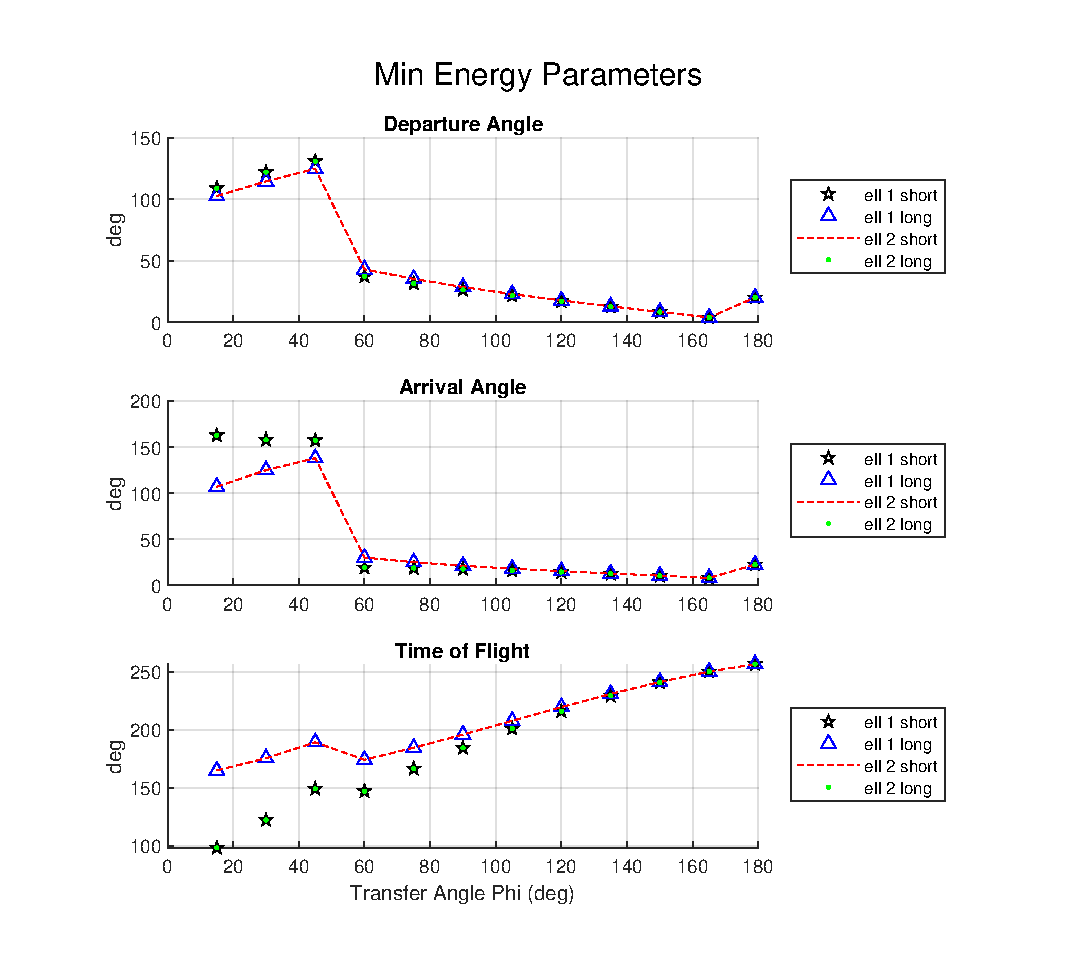
\includegraphics[width=0.8\textwidth]{phi15_180.pdf}
	\caption{Departure Angle, Arrival Angle, and TOF for Phi = 15 through 180 deg}
	\label{fig:phi_15_180}
\end{figure}


% 2.b 
\subsection*{B}
Discuss the significance of these plots for decision-making on the choice of
transfer angle and the semi-major axes of the transfer orbit.

\subsubsection*{Solution}

Lower departure and arrival angles may be desirable for a mission, as the delta-V required to enable capture by the destination planet's gravity would be lower. 


\newpage
% ================================================================ % 
\section*{Appendix} 

\subsection*{MATLAB code} 

\begin{lstlisting}
	%% HW 2 
	% Junette Hsin 
	
	% close all; 
	clear; 
	
	%% transfer angle = 75 deg 
	
	%  Define parameters for a state lookup:
	% t0      = 'Oct 20, 2020 11:00 AM CST'; 
	t0      = 'May 22, 1950'; 
	
	phi_t_des = 180; 
	[ell_1_min, ell_2_min, amin_AU, emin] = lambert_prob(t0, phi_t_des, 1); 
	
	
	%% phi = 15, 30, 45, 60, 75, 90, 105, 120, 135, 150, 165, 180 degrees
	
	phi_d_hist  = []; 
	phi_a_hist  = []; 
	tof_hist = []; 
	phi_t_hist = []; 
	
	phi0 = 15; 
	for phi = phi0 : 15 : 180 
		
		phi_t_des = phi; 
		[ell_1_min, ell_2_min] = lambert_prob(t0, phi_t_des, 0); 
		
		% departure angle: 
		% (1) ELL 1 SHORT, (2) ELL 1 LONG, (3) ELL 2 SHORT, (4) ELL 2 LONG 
		phi_d_hist = [phi_d_hist; ... 
			ell_1_min.phi_ds, ell_1_min.phi_dl, ell_2_min.phi_ds, ell_2_min.phi_dl]; 
	
		% arrival angle 
		% (1) ELL 1 SHORT, (2) ELL 1 LONG, (3) ELL 2 SHORT, (4) ELL 2 LONG 
		phi_a_hist = [phi_a_hist; ... 
			ell_1_min.phi_as, ell_1_min.phi_al, ell_2_min.phi_as, ell_2_min.phi_al]; 
	
		% time of flight 
		% (1) ELL 1 SHORT, (2) ELL 1 LONG, (3) ELL 2 SHORT, (4) ELL 2 LONG 
		tof_hist = [tof_hist; ... 
			ell_1_min.dt_s, ell_1_min.dt_l, ell_2_min.dt_s, ell_2_min.dt_l]; 
	
		% transfer angle 
		phi_t_hist = [phi_t_hist; phi_t_des]; 
			
		
	end 
	
	%%
	
	colors = {'k', 'b', 'r', 'g'}; 
	style = {'p', '^', '--', '.'}; 
	lwidth = [3, 1.5, 1, 1]; 
	
	figure()
		subplot(3,1,1) 
			hold on;
			for i = 1:4
	%             scatter(phi_t_hist, phi_d_hist(:,i), 4, colors{i});  
				h(i) = plot(phi_t_hist, phi_d_hist(:,i), [colors{i} style{i}]); 
			end 
			title('Departure Angle')
			ylabel('deg') 
			legend(h, 'ell 1 short', 'ell 1 long', 'ell 2 short', 'ell 2 long', 'location', 'eastoutside'); 
		
		subplot(3,1,2) 
			hold on;
			for i = 1:4
	%             scatter(phi_t_hist, phi_a_hist(:,i), 4, colors{i});  
				h(i) = plot(phi_t_hist, phi_a_hist(:,i), [colors{i} style{i}]); 
			end 
			title('Arrival Angle') 
			ylabel('deg') 
			legend(h, 'ell 1 short', 'ell 1 long', 'ell 2 short', 'ell 2 long', 'location', 'eastoutside'); 
			
		subplot(3,1,3) 
			hold on; 
			for i = 1:4
	%             scatter(phi_t_hist, tof_hist(:,i), 4, colors{i});  
				h(i) = plot(phi_t_hist, tof_hist(:,i), [colors{i} style{i}]); 
			end 
			title('Time of Flight') 
			ylabel('deg') 
			legend(h, 'ell 1 short', 'ell 1 long', 'ell 2 short', 'ell 2 long', 'location', 'eastoutside'); 
			
		xlabel('Transfer Angle Phi (deg)') 
	
		sgtitle('Min Energy Parameters') 
	
	%% save plots 
	
	
	%% RIGHT HERE 
function [ell_1_min, ell_2_min, amin_AU, emin] = lambert_prob(t0, phi_des, plot_option)

addpath(genpath('mice')); 
addpath(genpath('spice_data')); 

%  Load kernel file 
cspice_furnsh( 'spice_data/naif0011.tls' )
cspice_furnsh( 'spice_data/de421.bsp' )       
cspice_furnsh( 'spice_data/pck00010.tpc ') 

abcorr  = 'NONE';

%  Convert the epoch to ephemeris time (secs) 
et_t0   = cspice_str2et( t0 );

% get states --> Sun to Earth 
target   = 'Earth';
frame    = 'J2000';
observer = 'Sun';
abcorr   = 'NONE';

% get sun position 
et = et_t0;    % propagate ephemeris time by 1 day in secs 
X_sunE  = spice_state(et, target, frame, abcorr, observer); 

% get states --> Sun to Mars
target   = 'Mars';
frame    = 'J2000';
observer = 'Sun';
abcorr   = 'NONE';

% get sun position 
et = et_t0;    % propagate ephemeris time by 1 day in secs 
X_sunM  = spice_state(et, target, frame, abcorr, observer); 

% get angle between Earth and Mars velocities 
r_E = X_sunE(1:3); 
r_M = X_sunM(1:3); 
v_E = X_sunE(4:6); 
v_M = X_sunM(4:6); 

% angle and velocity angles 
phi_r = acosd( dot(r_E, r_M) / (norm(r_E)*norm(r_M)) ); 
phi_v = acosd( dot(v_E, v_M) / (norm(v_E)*norm(v_M)) ); 

i = 0; 
while abs(phi_r - phi_des) > 0.01
    
    % propagate by 0.1 day 
    i  = i + 0.01; 
    et = et_t0 + i*86400; 
    
    % get velocity 
    X_sunM  = spice_state(et, target, frame, abcorr, observer); 
    r_M = X_sunM(1:3); 
    v_M = X_sunM(4:6); 

    % get angle 
    phi_r = acosd( dot(r_E, r_M) / (norm(r_E)*norm(r_M)) ); 
    phi_v = acosd( dot(v_E, v_M) / (norm(v_E)*norm(v_M)) ); 
    
end 

% units in km 
rd_E = r_E ; 
ra_M = r_M ; 
vd_E = v_E ; 
va_M = v_M ; 

% propagate to get full Earth orbit 
X_sunE_hist = []; 
target   = 'Earth';
for i = 0:365+1
    
    et = et_t0 + i*86400; 
    
    % get state 
    X_sunE  = spice_state(et, target, frame, abcorr, observer); 
    
    % save Mars vector 
    X_sunE_hist = [X_sunE_hist; X_sunE]; 
end 

% propagate to get full Mars orbit 
X_sunM_hist = []; 
target   = 'Mars';
for i = 0:687+1
    
    et = et_t0 + i*86400; 
    
    % get state 
    X_sunM  = spice_state(et, target, frame, abcorr, observer); 
    
    % save Mars vector 
    X_sunM_hist = [X_sunM_hist; X_sunM]; 
end 

    
%% Part 1a
% Lambert - from VALLADO ed. 4, pgs 467 - 475 

% Arrival (Mars), AU units 
ra_mag = norm(ra_M); 
rd_mag = norm(rd_E); 

% Vallado method ... 
cos_dv = dot(rd_E, ra_M) / (rd_mag * ra_mag); 

% chord 
c = sqrt( rd_mag^2 + ra_mag^2 - 2*rd_mag*ra_mag*cos_dv ); 

% semiperimeter 
s = ( ra_mag + rd_mag + c ) / 2; 

% min semimajor axis 
amin = s/2;  

% initialize 
a_hist  = []; 

% 1 AU = km2AU km 
km2AU = 149598073; 

% loop 
for a = amin : 0.001*km2AU : 2*km2AU

    % time of flight 
    [ell_1, ell_2] = a2tof(s, c, a, rd_E, ra_M, vd_E, va_M); 
    
    % if 1st iteration, create ellipse hists 
    if a == amin 
        ell_1_hist = ell_1; 
        ell_2_hist = ell_2; 
        
    % else, build array 
    else 
        fnames = fieldnames(ell_1); 
        for i = 1:length(fnames)
            ell_1_hist.(fnames{i}) = [ell_1_hist.(fnames{i}); ell_1.(fnames{i})]; 
        end 
        fnames = fieldnames(ell_2); 
        for i = 1:length(fnames)
            ell_2_hist.(fnames{i}) = [ell_2_hist.(fnames{i}); ell_2.(fnames{i})]; 
        end 
    
    end 
    
    a_hist = [a_hist; a]; 
    
end 

% dt_hist_years = dt_hist / 365; 
a_hist_AU     = a_hist / km2AU; 

%% plot 

if plot_option > 0 
    
    fname = 'Ellipse 1 and 2 TOF and Angles'; 
    pos = [100 100 700 700]; 
    figure('name', fname, 'position', pos)
        subplot(3,1,1)
            plot(a_hist_AU, ell_1_hist.dt_s); hold on; 
            plot(a_hist_AU, ell_1_hist.dt_l); hold on; 
            plot(a_hist_AU, ell_2_hist.dt_s); hold on; 
            plot(a_hist_AU, ell_2_hist.dt_l); hold on; 
            legend('ell 1 short', 'ell 1 long', 'ell 2 short', 'ell 2 long', 'location', 'eastoutside'); 
            ylabel('TOF (days)') 
            title('a vs. TOF') 
        subplot(3,1,2) 
            plot(a_hist_AU, ell_1_hist.phi_ds); hold on; 
            plot(a_hist_AU, ell_1_hist.phi_dl); 
            plot(a_hist_AU, ell_2_hist.phi_ds); 
            plot(a_hist_AU, ell_2_hist.phi_dl); 
            legend('ell 1 short', 'ell 1 long', 'ell 2 short', 'ell 2 long', 'location', 'eastoutside')
            title('Ellipses 1 and 2: a vs. departure angles'); 
            ylabel('deg') 
        subplot(3,1,3) 
            plot(a_hist_AU, ell_1_hist.phi_as); hold on; 
            plot(a_hist_AU, ell_1_hist.phi_al); 
            plot(a_hist_AU, ell_2_hist.phi_as); 
            plot(a_hist_AU, ell_2_hist.phi_al); 
            legend('ell 1 short', 'ell 1 long', 'ell 2 short', 'ell 2 long', 'location', 'eastoutside')
            title('Ellipses 1 and 2: a vs. arrival angles'); 
            ylabel('deg') 
            xlabel('a (AU)'); 

        sgtitle(['Lambert Problem: \phi = ' num2str(phi_des) ' deg'])
    
end 

% [V1, V2] = LAMBERTBATTIN(rd, ra, 'retro', tof); 

%% propagate orbits 

if plot_option > 0 

a_ind = 160; 

fname = 'Ellipse 1 and 2, Short and Long'; 
pos   = [100 100 800 600]; 
figure('name', fname, 'position', pos)

    % subplot 1 
    subplot(2,2,1) 

        [rv_hist, oe_hist] = prop_probe ... 
            (ell_1_hist, rd_E, ra_M, 'short', a_ind);         
        ftitle = 'Ellipse 1 Short'; 
        plot_probe(rv_hist, X_sunE_hist, X_sunM_hist, rd_E, ra_M, ftitle) 
        
    % subplot 2 
    subplot(2,2,2) 

        [rv_hist, oe_hist] = prop_probe ... 
            (ell_1_hist, rd_E, ra_M, 'long', a_ind); 
        ftitle = 'Ellipse 1 Long'; 
        plot_probe(rv_hist, X_sunE_hist, X_sunM_hist, rd_E, ra_M, ftitle) 
    

    % subplot 3 
    subplot(2,2,3) 
    
        [rv_hist, oe_hist] = prop_probe ... 
            (ell_2_hist, rd_E, ra_M, 'short', a_ind);         
        ftitle = 'Ellipse 2 Short'; 
        plot_probe(rv_hist, X_sunE_hist, X_sunM_hist, rd_E, ra_M, ftitle) 

    % subplot 4 
    subplot(2,2,4) 
    
        [rv_hist, oe_hist] = prop_probe ... 
            (ell_2_hist, rd_E, ra_M, 'long', a_ind);         
        ftitle = 'Ellipse 2 Long'; 
        plot_probe(rv_hist, X_sunE_hist, X_sunM_hist, rd_E, ra_M, ftitle) 

    sgtitle(['Lambert Problem: \phi = ' num2str(phi_des) ' deg'])
    
end 

%% minimum energy transfer orbit 

pmin = rd_mag*ra_mag/c * (1 - cosd(phi_r)); 
emin = sqrt( 1 - 2*pmin/s ); 
amin_AU = amin / km2AU; 

sprintf('a_min = %.5g AU, e_min = %.5g', amin_AU, emin)

[ell_1_min, ell_2_min] = a2tof(s, c, amin, rd_E, ra_M, vd_E, va_M); 


end 


%% subfunctions 

function plot_probe(rv_hist, X_sunE_hist, X_sunM_hist, rd_E, ra_M, ftitle) 

    z_rv = zeros(length(rv_hist), 1); 
    z_E  = zeros(length(X_sunE_hist), 1); 
    z_M  = zeros(length(X_sunM_hist), 1); 

    plot3([z_rv rv_hist(:,1)], [z_rv rv_hist(:,2)], [z_rv rv_hist(:,3)], 'g', 'linewidth', 2); 
    hold on; 
    scatter3([rd_E(1)], [rd_E(2)], [rd_E(3)], 80, 'go', 'linewidth', 2 );
    scatter3([ra_M(1)], [ra_M(2)], [ra_M(3)], 80, 'g^', 'linewidth', 2 ); 
    plot3([z_E X_sunE_hist(:,1)], [z_E X_sunE_hist(:,2)], [z_E X_sunE_hist(:,3)], 'b--')
    plot3([z_M X_sunM_hist(:,1)], [z_M X_sunM_hist(:,2)], [z_M X_sunM_hist(:,3)], 'r--')
    title(ftitle)
    xlabel('x (km)'); ylabel('y (km)'); zlabel('z (km)'); 

end 

function [rv_hist, oe_hist] = prop_probe (ell_x_hist, rd, ra, dt_str, a_ind)

    % probe orbit (min energy) 
    if strcmp(dt_str, 'short')
        vd = ell_x_hist.vd_s(a_ind,:); 
        va = ell_x_hist.va_s(a_ind,:); 
        dt = ell_x_hist.dt_s(a_ind); 
    elseif strcmp(dt_str, 'long')
        vd = ell_x_hist.vd_l(a_ind,:); 
        va = ell_x_hist.va_l(a_ind,:); 
        dt = ell_x_hist.dt_l(a_ind);         
    else
        disp('Choose long or short')
        return 
    end 

    % sun mu (m^3/s^2)
    mu_sun_m = 1.32712440018e20; 
    mu_sun_km = mu_sun_m / (1000^3); 

    % probe state in km 
    X_probe0 = [rd'; vd']; 
    oe_probe0 = rvOrb.rv2orb(X_probe0, mu_sun_km); 
    X_probef = [ra'; va']; 
    oe_probef = rvOrb.rv2orb(X_probef, mu_sun_km); 

    % delta anomaly 
    dM = oe_probef(6) - oe_probe0(6); 
    if strcmp(dt_str, 'long')
        dM = 2*pi - dM; 
    end 

    % mean motion (rad/days) 
    n  = dM / dt; 
    if strcmp(dt_str, 'long')
        n = -n;  
    end 

    % propagate orbit 
    oe_hist = oe_probe0; 
    rv_hist = [X_probe0']; 
    for i = 1:round(dt)

        oe = oe_probe0; 

        % propagate nu by i days 
        nu = oe_probe0(6) + n*i; 
        oe(6) = nu; 

        % convert to cartesian 
        rv = rvOrb.orb2rv(oe, mu_sun_km); 

        oe_hist = [oe_hist; oe]; 
        rv_hist = [rv_hist; rv']; 

    end 

end 

function [ell_1, ell_2] = a2tof(s, c, a, rd, ra, vd_E, va_M)
% ------------------------------------------------------------------------
% Inputs: 
%   s = semiperimeter (km) 
%   c = chord (km) 
%   a = semimajor axis (km) 
% 
% Outputs: 
%   ellipse 1 
%   ellipse 2 
%       each containing: 
%           TOF for short and long 
%           departure velocities for short and long 
%           arrival velocities for short and long 
%           departure angles for short and long 
%           arrival angles for short and long 
% ------------------------------------------------------------------------

% time of flight 
alpha1 = 2 * asin( sqrt( s/(2*a) ) ); 
alpha2 = 2*pi - alpha1; 
beta1  = 2 * asin( sqrt( (s-c)/(2*a) ) ); 
beta2  = - beta1; 

% sun mu (m^3/s^2)
mu_sun_m = 1.32712440018e20; 
mu_sun_km = mu_sun_m / (1000^3); 

% time of flight 
nrev = 0; 
dt1_s = sqrt( a^3/mu_sun_km ) * ... 
    (( 2*nrev*pi + alpha1 - sin(alpha1) - (beta1 - sin(beta1)) )); 
dt1_l = sqrt( a^3/mu_sun_km ) * ... 
    (( 2*nrev*pi + alpha1 - sin(alpha1) + (beta1 - sin(beta1)) )); 
dt2_s = sqrt( a^3/mu_sun_km ) * ... 
    (( 2*nrev*pi + alpha2 - sin(alpha2) - (beta2 - sin(beta2)) )); 
dt2_l = sqrt( a^3/mu_sun_km ) * ... 
    (( 2*nrev*pi + alpha2 - sin(alpha2) + (beta2 - sin(beta2)) )); 

% convert from seconds to days 
day2sec = 60*60*24; 

ell_1.dt_s = dt1_s / day2sec; 
ell_1.dt_l = dt1_l / day2sec; 
ell_2.dt_s = dt2_s / day2sec; 
ell_2.dt_l = dt2_l / day2sec; 

% ------------------------------------------------------------------------
% VELOCITIES 

% geometry 
rd_mag = norm(rd); 
ra_mag = norm(ra); 
dnu = acos( dot(rd, ra) / ( rd_mag*ra_mag ) ); 
de = alpha1 - beta1; 

% commented out failed velocity code 

% June Battin 
[vd1_s, va1_s] = LAMBERTBATTIN_km_sun_June(rd, ra, 'pro', dt1_s); 
[vd1_l, va1_l] = LAMBERTBATTIN_km_sun_June(rd, ra, 'pro', dt1_l); 
[vd2_s, va2_s] = LAMBERTBATTIN_km_sun_June(rd, ra, 'pro', dt2_s); 
[vd2_l, va2_l] = LAMBERTBATTIN_km_sun_June(rd, ra, 'pro', dt2_l); 

ell_1.vd_s = vd1_s; 
ell_1.va_s = va1_s; 
ell_1.vd_l = vd1_l; 
ell_1.va_l = va1_l; 
ell_2.vd_s = vd2_s; 
ell_2.va_s = va2_s; 
ell_2.vd_l = vd2_l; 
ell_2.va_l = va2_l; 

% ------------------------------------------------------------------------
% ANGLES 
    
% ELLIPSE 1 departure angle, short and long  
vd_s = ell_1.vd_s; 
phi1_ds = acosd( dot(vd_s, vd_E) / ( norm(vd_s)*norm(vd_E) ) ); 
vd_l = ell_1.vd_l; 
phi1_dl = acosd( dot(vd_l, vd_E) / ( norm(vd_l)*norm(vd_E) ) ); 

ell_1.phi_ds = phi1_ds; 
ell_1.phi_dl = phi1_dl; 

% ELLIPSE 1 arrival angle, short and long  
va_s = ell_1.va_s; 
phi1_as = acosd( dot(va_s, va_M) / ( norm(va_s)*norm(va_M) ) ); 
va_l = ell_1.va_l; 
phi1_al = acosd( dot(va_l, va_M) / ( norm(va_l)*norm(va_M) ) ); 

ell_1.phi_as = phi1_as; 
ell_1.phi_al = phi1_al; 

% ELLIPSE 2 departure angle, short and long  
vd_s = ell_2.vd_s; 
phi2_ds = acosd( dot(vd_s, vd_E) / ( norm(vd_s)*norm(vd_E) ) ); 
vd_l = ell_2.vd_l; 
phi2_dl = acosd( dot(vd_l, vd_E) / ( norm(vd_l)*norm(vd_E) ) ); 

ell_2.phi_ds = phi2_ds; 
ell_2.phi_dl = phi2_dl; 

% ELLIPSE 2 arrival angle, short and long  
va_s = ell_2.va_s; 
phi2_as = acosd( dot(va_s, va_M) / ( norm(va_s)*norm(va_M) ) ); 
va_l = ell_2.va_l; 
phi2_al = acosd( dot(va_l, va_M) / ( norm(va_l)*norm(va_M) ) ); 

ell_2.phi_as = phi2_as; 
ell_2.phi_al = phi2_al; 

end 

%% Gauss solution 

function [vd, va] = lambert_gauss(rd, ra, dt1_s, mu_sun_km, de)

rd_mag = norm(rd); 
ra_mag = norm(ra); 
dnu = acos( dot(rd, ra) / ( rd_mag*ra_mag ) ); 

% Gauss solution 
L = (rd_mag + ra_mag) / ( 4*sqrt( rd_mag*ra_mag ) * cos(dnu/2) ) - 1/2;  
m = mu_sun_km * dt1_s^2 / ( 2*sqrt(rd_mag*ra_mag) * cos(dnu/2) )^3; 

yold = 0; 
ynew = 1; 

while abs(yold - ynew) > 0.001
    yold = ynew; 
    x1 = m / yold^2 - L; 
    x2 = (de - sin(de)) / ( sin(de/2) )^3; 
    ynew  = (L + x1)*x2 + 1; 
end 

cos_de2 = 1 - 2*x1; 
p = rd_mag*ra_mag*(1 - cos(dnu)) / ... 
    ( rd_mag + ra_mag - 2*sqrt(rd_mag*ra_mag)*cos(dnu/2)*cos_de2 ); 

f = 1 - ra_mag/p * ( 1-cos(dnu) ); 
g = ra_mag*rd_mag * sin(dnu) / sqrt( mu_sun_km * p );

df = sqrt(1/p) * tan(dnu/2) * ( ( 1-cos(dnu) )/p - 1/ra_mag - 1/rd_mag ); 
dg = 1 - rd_mag/p * (1-cos(dnu)); 

vd = (ra - f*rd)/g; 
va = (dg*ra - rd)/g; 

end 

%% Kepler equation solver 

function E = keplerEq(M,e,eps)
% Function solves Kepler's equation M = E-e*sin(E)
% Input - Mean anomaly M [rad] , Eccentricity e and Epsilon 
% Output  eccentric anomaly E [DEG]. 
   	En  = M;
	Ens = En - (En-e*sind(En)- M)/(1 - e*cosd(En));
	while ( abs(Ens-En) > eps )
		En = Ens;
		Ens = En - (En - e*sind(En) - M)/(1 - e*cosd(En));
    end
	E = Ens;
end

function E = kepler(M, e)
    f = @(E) E - e * sind(E) - M;
    E = fzero(f, M);  % <-- I would use M as the initial guess instead of 0
end

%% annotation 

function h_text(h2, text1, text2, text3, text4) 

    pos = get(h2, 'position');     
    delete(findall(gcf,'type','annotation')); 
    text = { ''; ''; text1; text2; text3; text4 }; 
    annotation('textbox', pos, ...
      'String', text, ...
      'edgecolor', 'none');
    axis off 

end 

%% commented out failed velocity code 

% % Battin solution (definitely works) 
% % ellipse 1, long and short 
% [vd1_s, va1_s] = LAMBERTBATTIN_km_sun(rd, ra, 'pro', dt1_s); 
% [vd1_l, va1_l] = LAMBERTBATTIN_km_sun(rd, ra, 'pro', dt1_l); 
%  
% % ellipse 2, long and short 
% [vd2_s, va2_s] = LAMBERTBATTIN_km_sun(rd, ra, 'pro', dt2_s); 
% [vd2_l, va2_l] = LAMBERTBATTIN_km_sun(rd, ra, 'pro', dt2_l); 
% 
% compute velocities - Bettadpur and Vallado combination 
% n  = @(alpha1, beta1, dt1_s) ...  
%         (alpha1 - beta1) - 2*cos( (alpha1+beta1)/2 )*sin( (alpha1-beta1)/2 ); 
% f  = @(alpha1, beta1) ... 
%         1 - a/rd_mag * ( 1 - cos(alpha1 - beta1) ); 
% g  = @(alpha1, beta1, dt1_s) ... 
%         dt1_s - 1/n(alpha1, beta1, dt1_s) * ( de - sin(alpha1 - beta1) ); 
% 
% K  = 4*a/c^2 * ( 1/2*(rd_mag+ra_mag+c) - rd_mag ) * ( 1/2*(rd_mag+ra_mag+c) - ra_mag ); 
% p1 = @(alpha1, beta1) ... 
%         K * sin( (alpha1+beta1)/2 )^2; 
% p2 = @(alpha1, beta1) ... 
%         K * sin( (alpha1-beta1)/2 )^2; 
% 
% dg = @(alpha1, beta1, p1) ... 
%         1 - rd_mag/p1(alpha1, beta1) * ( 1-cos(dnu) ); 
% vd1_s = ( ra - f(alpha1, beta1)*rd ) / ... 
%             g(alpha1, beta1, dt1_s);
% vd1_l = - vd1_s; 
% vd2_s = ( ra - f(alpha2, beta2)*rd ) / ... 
%             g(alpha2, beta2, dt2_s);
% vd2_l = - vd2_s; 


% va2_s = ( dg(alpha2, beta2, p2)*ra - rd ) / ... 
%             g(alpha2, beta2, dt2_s); 
% vd2_l = ( ra - f(alpha2, beta2)*rd ) / ... 
%             g(alpha2, beta2, dt2_l);
% va2_l = ( dg(alpha2, beta2, p2)*ra - rd ) / ... 
%             g(alpha2, beta2, dt2_l); 

% Gauss solution 
% [vd1_s_gauss, va1_s_gauss] = lambert_gauss(rd, ra, dt1_s, mu_sun_km, de); 
% [vd1_l_gauss, va1_l_gauss] = lambert_gauss(rd, ra, dt1_l, mu_sun_km, de); 
% [vd2_s_gauss, va2_s_gauss] = lambert_gauss(rd, ra, dt2_s, mu_sun_km, de); 
% [vd2_l_gauss, va2_l_gauss] = lambert_gauss(rd, ra, dt2_l, mu_sun_km, de); 

% Universal variables 
% A = sqrt(ra_mag*rd_mag)*sin(dnu) / ( sqrt( 1 - cos(dnu) ) ); 
% psi_n = 0; 
% c2 = 1/2; 
% c3 = 1/6; 
% psi_up  = 4*pi^2; 
% psi_low = -4*pi; 
% 
% dtn = 1; 
% while abs( dtn - dt1_s ) > 0.01
%     
%     yn = rd_mag + ra_mag + A*(psi_n*c3 - 1)/sqrt(c2); 
%     if A > 0 && yn < 0 
%         psi_low = psi_low + 0.01; 
%     end 
%     
%     xn = sqrt(yn/c2); 
%     dtn = (xn^3*c3 + A*sqrt(yn)) / (sqrt(mu_sun_km)); 
%     
%     if dtn < dt1_s
%         psi_n = psi_low; 
%     else
%         psi_n = psi_up; 
%     end 
%     
%     psi_np1 = (psi_up + psi_low)/2; 
%     
%     % find c2 and c3 
%     
%     psi_n = psi_np1; 
%     
% end 


function [vd, va] = LAMBERTBATTIN_km_sun_June(rd, ra, dm, dt)
% VALLADO BATTIN METHOD 

% mu = 3.986004418e14;   % m3/s2
mu_sun_m = 1.32712440018e20; 
mu_sun_km = mu_sun_m / (1000^3); 
mu = mu_sun_km; 

% cos and sin dnu 
ra_mag  = norm(ra);
rd_mag  = norm(rd);
cos_dnu = dot(rd,ra)/(rd_mag*ra_mag);
dnu     = acos(cos_dnu); 
sin_dnu = sin(dnu); 

% the angle needs to be positive to work for the long way
if dnu < 0.0
    dnu = 2*pi + dnu;
end

% geometry 
c   = sqrt( rd_mag^2 + ra_mag^2 - 2*rd_mag*ra_mag*cos_dnu ); 
s   = ( rd_mag + ra_mag + c ) / 2; 
eps = (ra_mag - rd_mag) / rd_mag; 

% tan2w --> rdp 
sqrt_rda = sqrt( ra_mag / rd_mag ); 
tan22w    = ( eps^2/4 ) / ( sqrt_rda + sqrt_rda^2*( 2 + sqrt_rda ) ); 
rdp      = sqrt( rd_mag*ra_mag ) * ( cos( dnu/4 )^2 + tan22w ); 

% obtain L 
if dnu < pi 
    num = sin(dnu/4)^2 + tan22w; 
    den = sin(dnu/4)^2 + tan22w + cos(dnu/2); 
else
    num = cos(dnu/4)^2 + tan22w - cos(dnu/2); 
    den = cos(dnu/4)^2 + tan22w; 
end 
L = num / den; 

m = mu * dt^2 / ( 8*rdp^3 ); 

% orbit is elliptical 
xn = L;
eta = xn / ( sqrt( 1+xn ) + 1 )^2;  
x = -xn; 

i = 0; 
% loop 
while (1) 
    
    i = i + 1; 
    
    x = xn; 
    
    % omg crazy recursion in fraction denominator 
    tempx = seebatt(x); 

    % h1 
    num = (L+x)^2 * (1 + 3*x + tempx); 
    den = ( 1 + 2*x + L ) * ( 4*x + tempx*( 3+x ) ); 
    h1  = num / den; 
    
    % h2 
    num = m*(x - L + tempx); 
    h2  = num / den; 
    
    % solve cubic y^3 - y^2 - h1*y^2 - h2 = 0 
    rts = roots([1 -1 -h1 -h2]); 
    
    B = 27*h2 / ( 4*( 1 + h1 )^3 ); 
    U = B / ( 2*( sqrt( 1+B ) + 1 ) ); 
    
    K = seebattk(U); 
    y = (1 + h1)/3 * ( 2 + ( sqrt(1+B) )/( 1 + 2*U*K^2 ) ); 
    xn = sqrt( ( (1-L)/2 )^2 + ( m/y^2 ) ) - (1+L)/2; 
    
    if abs(xn - x) < 0.000001 && i > 30
        break 
    end 
        
end 

% semi-major axis!!! 
a = mu_sun_km*dt^2 / ( 16 * rdp^2 * x * y^2 ); 

if a > 0 
    
    % obtain f, g, and dg 
    alpha = 2 * asin( sqrt( s/(2*a) ) ); 
    beta  = 2 * asin( sqrt( (s-c)/(2*a) ) ); 
    
    % min 
    amin = s / 2; 
    tmin = sqrt( amin^3/mu_sun_km ) * ( pi - beta + sin(beta) ); 
    if dt > tmin 
        alpha = 2*pi - alpha; 
    end 
    de    = alpha - beta; 
    
    f  = 1 - a/rd_mag * ( 1 - cos(de) ); 
    g  = dt - sqrt( a^3/mu_sun_km ) * ( de - sin(de) ); 
    dg = 1 - a/ra_mag * ( 1 - cos(de) ); 

else
    
    disp('oh no') 
    
end 

% velocities!! 
vd = (ra - f*rd) / g; 
va = (dg*ra - rd) / g; 

end 
	
	
	
	
\end{lstlisting}





% ================================================================ % 

% \bibliography{sample}

\end{document}
